\chapter{Mechanizmy Bezpieczeństwa}

Bezpieczeństwo to fundamentalny aspekt systemów uwierzytelniania. \textbf{FaceAuthApp} posiada kompleksowy zbiór mechanizmów chroniących przed popularnymi atakami (jak chociażby przyłożenie zdjęcia do kamery) oraz zapewniających pełną śledzalność logowań w architekturze korporacyjnej.

\section{Analiza Żywotności Obiektu (Liveness Detection / Anti-Spoofing)}
Jednym z najczęstszych ataków na podstawowe systemy biometryczne jest tzw. atak prezentacyjny (Presentation Attack / Spoofing). Intruz podstawia przed obiektyw kamery wydrukowane na kartce papieru zdjęcie twarzy ofiary, lub wyświetla jej podobiznę na ekranie telefonu.

Dla ochrony przed tym typem ataku, algorytm logowania aplikacji wymusza analizę mikro-ruchów obiektu poprzez badanie wariancji kolorów na klatkach z opóźnieniem czasowym:
\begin{itemize}
    \item System nie rejestruje obrazu natychmiast po wciśnięciu przycisku logowania. Zamiast tego przechwytuje \textbf{trzy osobne klatki} w krótkich odstępach czasu (około 300 milisekund przerw).
    \item Zebrany materiał jest porównywany pod kątem drobnych przemieszczeń pikseli w rejonie centralnym kadru (obszar twarzy).
    \item Algorytm bada różnice w naświetleniu i przesunięciu wartości RGB. Sumuje on wariancję między klatką pierwszą a drugą, a następnie dołącza zmianę względem klatki trzeciej.
    \item Jeśli wynik wariancji wynosi niemal zero (współczynnik poniżej progu 10), obiekt jest absolutnie statyczny – system wykrywa atak i generuje komunikat \textit{"Zablokowano: Wykryto oszustwo (Statyczny Obraz)"}, blokując wejście na proces analizy modelu sztucznej inteligencji.
\end{itemize}

\section{Logi Audytowe (Audit Trail)}
Każda akcja w systemie pozostawia bezpieczny, trudny do zmodyfikowania w normalnym toku ślad w wbudowanym pliku tekstowym \texttt{Security\_Audit.log}. Zapis realizowany jest w modelu append-only i rejestruje dokładny stempel czasowy, status próby autoryzacyjnej, ostatecznie wyliczony wskaźnik podobieństwa Score, oraz szczegółową wiadomość dla administratora systemu. Wyróżniamy 3 rodzaje wpisów:
\begin{itemize}
    \item \textbf{GRANTED:} Skuteczne i pomyślne logowanie konkretnego użytkownika.
    \item \textbf{DENIED:} Odmowa dostępu (nieprzekroczony wymagany próg Score, lub wczesne odrzucenie za próbę oszustwa statycznym obrazkiem).
    \item \textbf{ERROR:} Śledzenie wyjątków sprzętowych (np. utrata zasilania kamery, błędy alokacji modelu w pamięci).
\end{itemize}

\begin{center}
    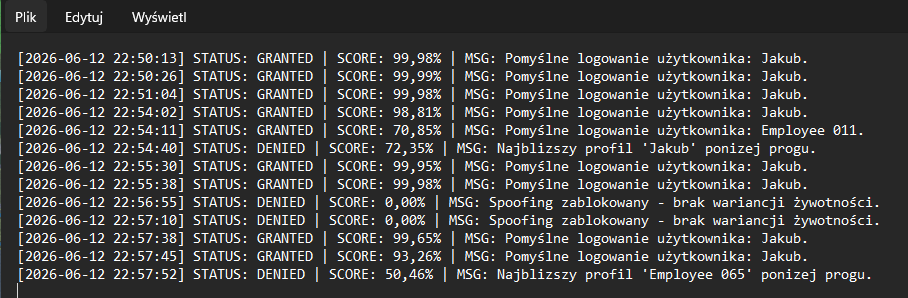
\includegraphics[width=0.55\textwidth]{img/ui/audit_log.png}
    \captionof{figure}{Wycinek z logów \texttt{Security\_Audit.log} dokumentujący udane i odrzucone próby autoryzacyjne w systemie.}
\end{center}

\section{Kwarantanna dla Intruzów (Snapshots)}
Zastosowanie rygorystycznej polityki obronnej pozwoliło na implementację procedury zapisywania dowodów incydentów bezpieczeństwa. 
Gdy niezidentyfikowana osoba podda się procesowi uwierzytelniania, a silnik wskaże negatywny wynik dopasowania profilu (poniżej wartości brzegowej \textit{Threshold}), wizerunek tej osoby zostaje błyskawicznie przechwycony. Obraz jest następnie trwale archiwizowany na dysku, w dedykowanym podfolderze \texttt{Zagrożenia}, przyjmując unikalną nazwę np. \texttt{INTRUZ\_20260601\_153000.jpg}. Chroni to placówkę fizycznie przed nieuprawnionym dostępem i ułatwia późniejsze dochodzenia wewnętrzne.

\begin{center}
    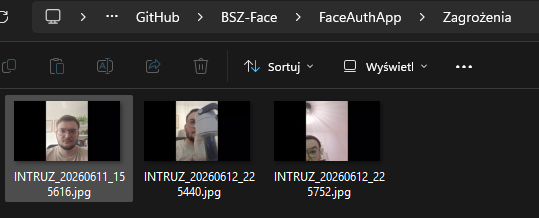
\includegraphics[width=0.55\textwidth]{img/ui/intruder_folder.png}
    \captionof{figure}{Archiwum przechwyconych zdjęć intruzów, u których poziom weryfikacji spadł poniżej zadanego progu.}
\end{center}
